
Um bestimmte Darstellungskomponenten, im weiteren als Plugins bezeichnet, in das UI (in unserem Fall die Website) einzubinden, wird das MVC-Pattern verwendet. Solche Plugins können z.B. die Ausgabe von Ergebnissen als Text oder Grafik sein, aber auch Eingabemasken zum Erstellen von Modellen. 

\begin{figure}[h]
\centering
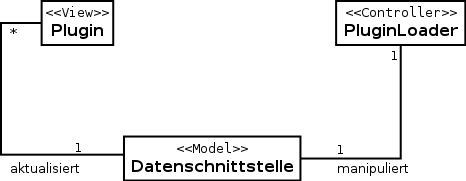
\includegraphics[width=0.6\linewidth]{Grafik/Diagramm/Pattern/MVC/Kontextdiagramm.png}
\caption[MVC Website Klassen]{MVC-Pattern zum Website anzeigen}
\end{figure}

\noindent Sollte der Benutzer z.B. ein Modell generieren wollen oder sich ein Ergebnis anzeigen lassen, so formuliert der PluginLoader eine Anfrage an die Datenschnittstelle, um mögliche Änderungen an diese zu senden. Nach diesem Aktualisierungsprozess wird ein Plugin durch den PluginLoader generiert, das über die Datenschnittstelle die notwendigen Informationen bezieht. Sollten hierbei Anfragen an andere Server nötig sein, so werden diese ebenfalls von der Datenschnittstelle mittels des REST-Protokolls durchgeführt. Das fertige Plugin wird nun in das Haupt-UI integriert.

\begin{figure}[h]
\centering
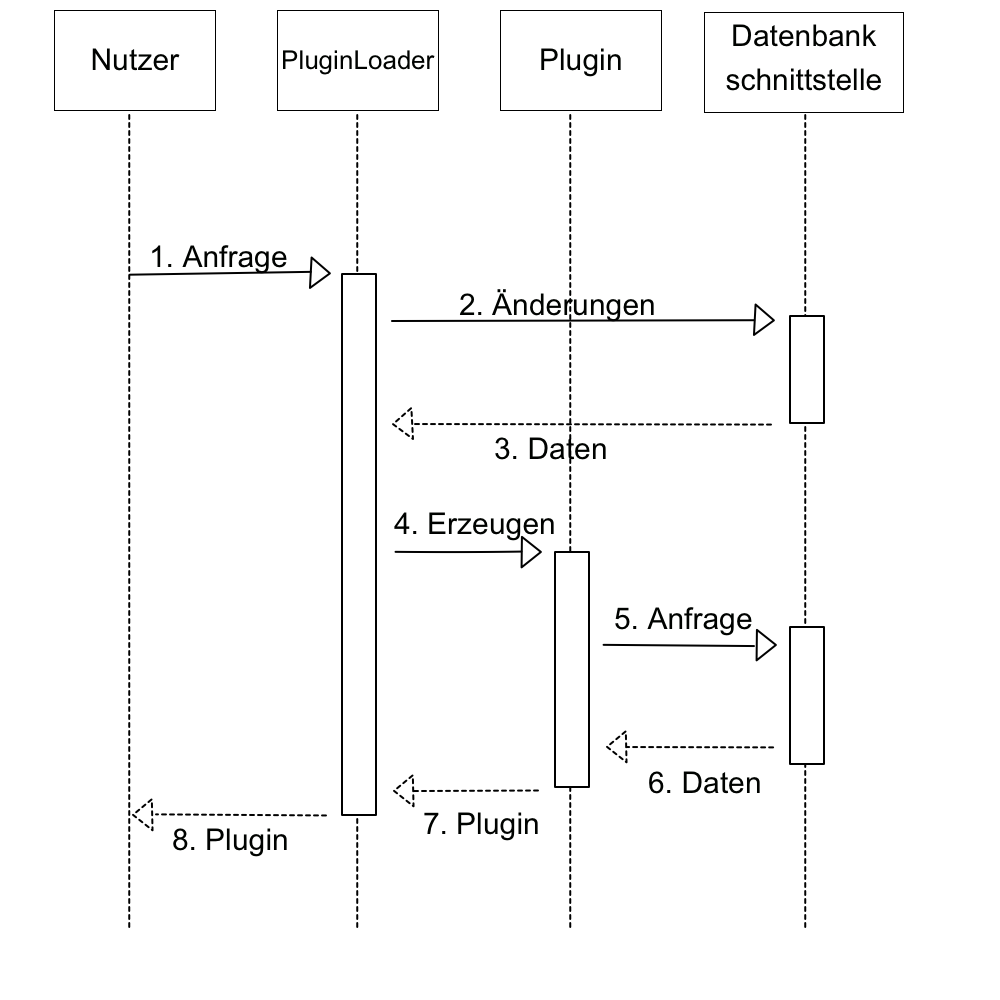
\includegraphics[width=0.6\linewidth]{Grafik/Diagramm/Pattern/MVC/Sequenzdiagramm.png}
\caption[MVC Website Sequenz]{MVC-Pattern Sequenz zum Generieren der Website}
\end{figure}

\subsubsection{Was spricht für Model-View-Controller?}
Das MVC-Pattern ermöglicht es, das System leicht zu erweitern. 
Durch die Einbindung verschiedener Plugins in das System wird gewährleistet, dass auf neue Gegebenheiten schnell reagiert werden kann.
Sollte z.B. ein Algorithmus eine spezifische Ausgabe benötigen, könnte speziell für diesen ein neues Plugin erstellt werden. 
Des Weiteren erleichtert diese Aufteilung die Wartung des Systems enorm, da einzelne Plugins für sich getestet werden können, ohne in das Gesamtsystem eingebettet zu sein. 

